\documentclass[graphics]{beamer}

\usepackage{graphicx}
\usepackage{verbatim}
\usepackage{wrapfig}
\usepackage{multimedia}
\useoutertheme{shadow}
%\usecolortheme{orchid}
\usecolortheme{seahorse}


% math commands
\newcommand{\be}{\begin{eqnarray}}
\newcommand{\ee}{\end{eqnarray}}
\newcommand{\beq}{\begin{equation}}
\newcommand{\eeq}{\end{equation}}
\def\simless{\mathbin{\lower 3pt\hbox
      {$\rlap{\raise 5pt\hbox{$\char'074$}}\mathchar"7218$}}}
\def\simgreat{\mathbin{\lower 3pt\hbox
      {$\rlap{\raise 5pt\hbox{$\char'076$}}\mathchar"7218$}}} %> or of order

% variables

\def\toonscale{0.45}
\def\mboxy#1{\mbox{\small #1}}


\begin{comment}
\AtBeginSection[]{
  \frame{
    \frametitle{Outline}
    \tableofcontents[currentsection]
  }
}
\end{comment}

\title{New Window on the Universe through FRBs}
%\subtitle{interim update}
\author[U. Pen]{Ue-Li Pen and collaborators
}
\date{January 27, 2025}


\begin{document}

%\section*{Introduction}
\section{FRBs}

\begin{comment}
  \subsection{Outline}

  \frame{
    \frametitle{Outline}
    \tableofcontents
  }
\end{comment}

\frame{\maketitle}


  \frame{
    \frametitle{Fast Radio Bursts}
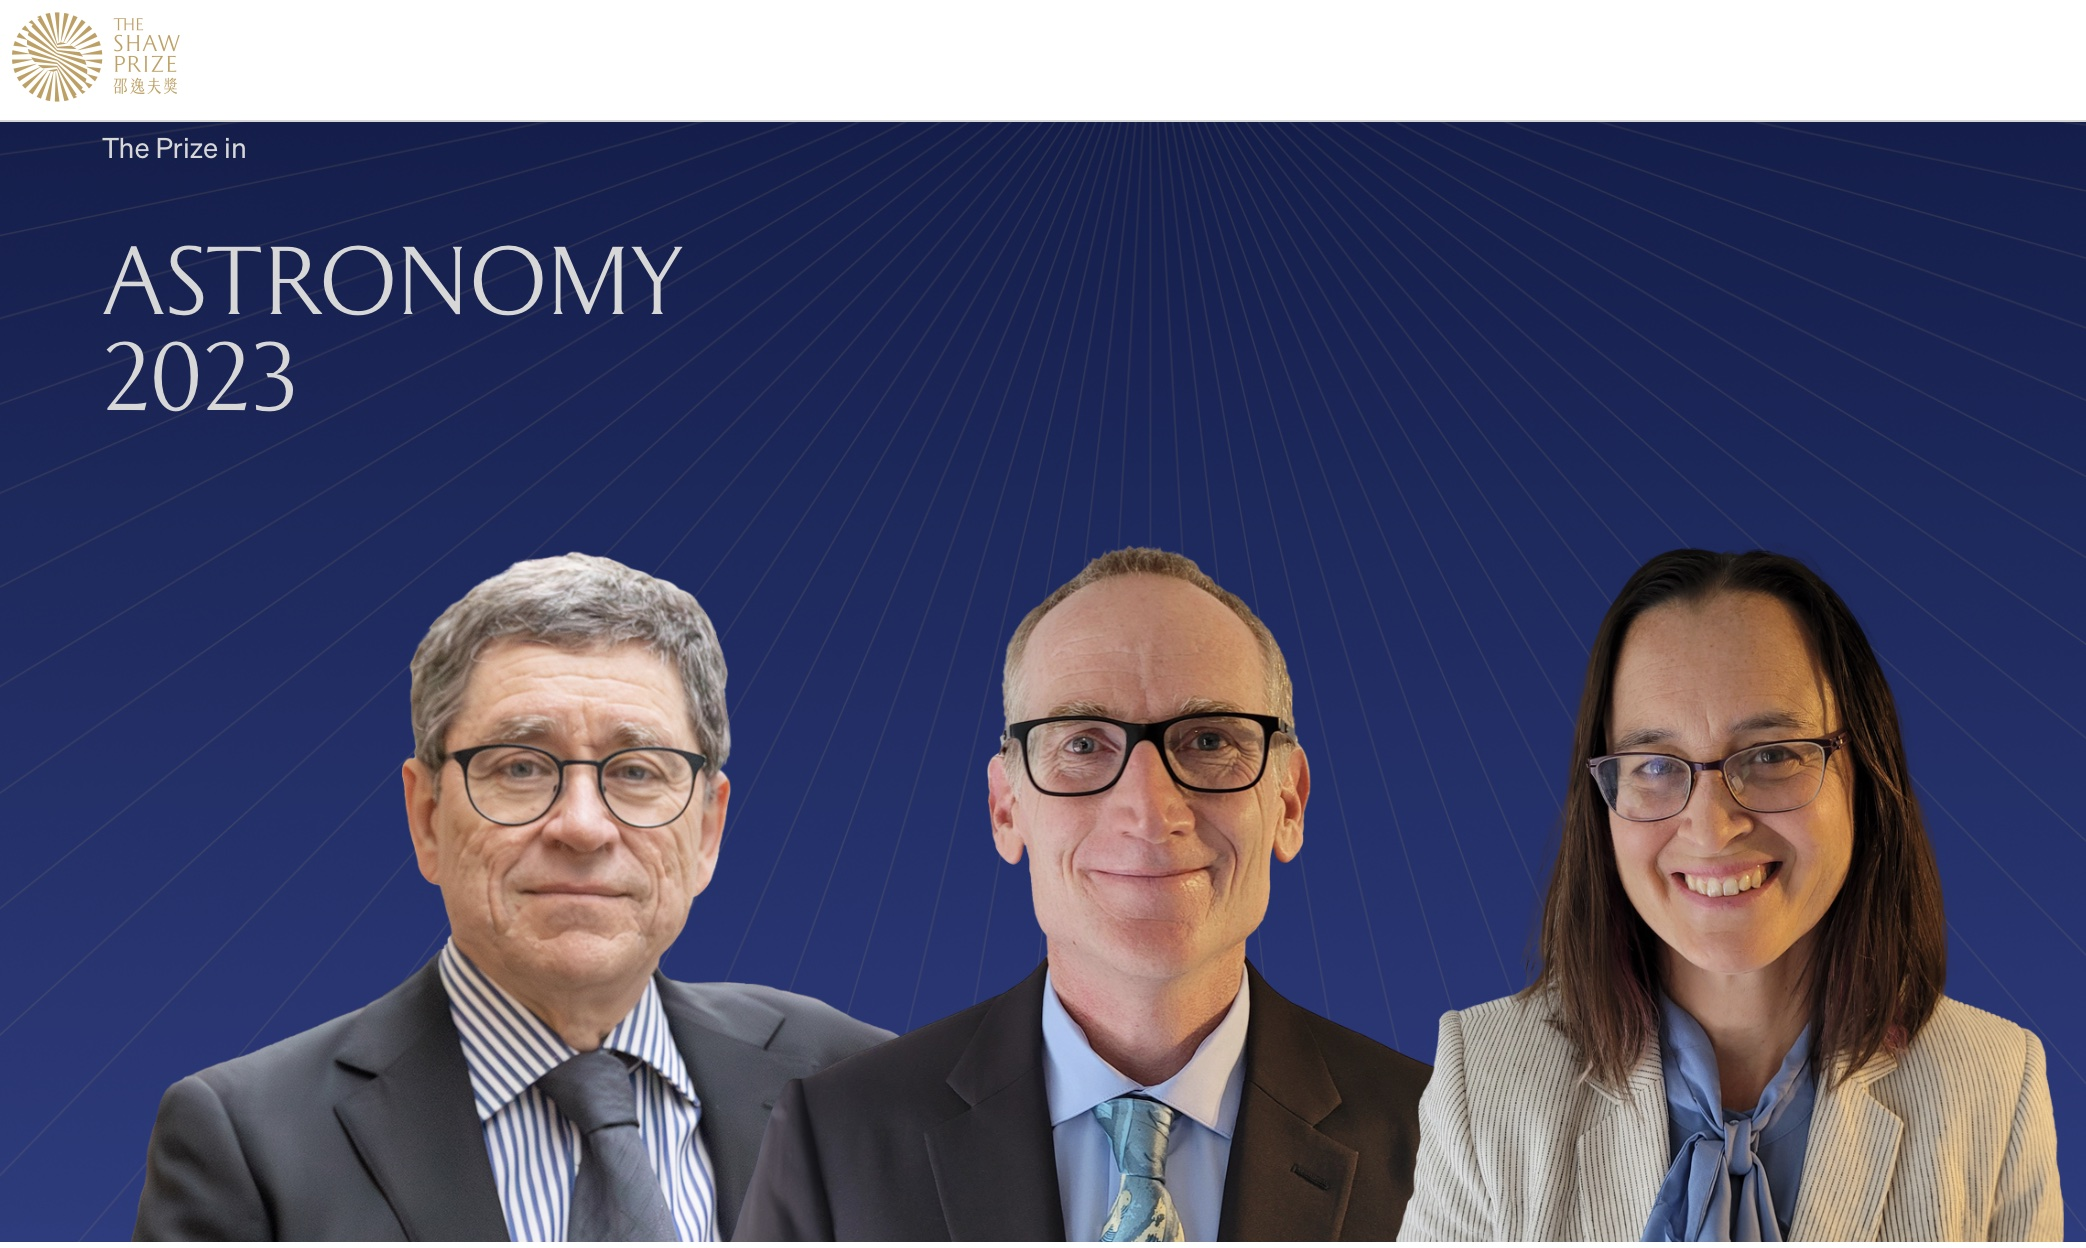
\includegraphics[width=4.5in]{Figures/shaw2023.jpg}
  }


  \frame{
    \frametitle{Fast Radio Bursts}
\small

The Shaw Prize in Astronomy 2023 is awarded in equal shares to {\bf Matthew
Bailes, Duncan Lorimer}, and {\bf Maura McLaughlin} the discovery of fast
radio bursts (FRBs).

FRBs are among the most extreme and mysterious phenomena in astronomy:
they are intense bursts of radio emission lasting only a few
thousandths of a second that contain as much energy as the Sun emits
over several days. The sources of the bursts are smaller than the
Earth but are as far away as distant galaxies. In a seminal research
paper written in 2007, Bailes, Lorimer, McLaughlin (with collaborators
Narkevic and Crawford) found the first FRB; deduced many of the
properties of its source, in particular its extreme distance, small
size, and enormous energy; estimated the cosmic rate of production of
FRBs; and highlighted their potential as cosmological probes.

  }


  \frame{
\vspace{-0.25in}
    \frametitle{FRB110523}
 

%\hspace{2.5in}
\includegraphics[width=2.5in]{Figures/scint110523.png}
\includegraphics[width=1.75in]{Figures/corr110523.png}

Masui+ULP++ 2015, Nature, 528, 523
  }



  \frame{
    \frametitle{Fast Radio Bursts}
    \begin{itemize}
        \item Interference effects under multi-path propagation: same
          class as GWs
        \item potential for diffraction limited measurements: cosmic distances
        \item BURSTT
    \end{itemize}
  }

  \frame{
    \frametitle{FRBs}
    \begin{itemize}
      \item thousands detected
      \item increasing sample of well-localized FRBs
        \item Coherent, distant source of radiation
        \item Scintillate under multi-path propagation          
        \item sensitive to ns time delay propagating for gigaparsecs
        \item corresponds to strain $h \ll 10^{-26}$: far exceeds LIGO
        \item highly elongated antenna pattern: sensitive to
          longitudinal modes          
    \end{itemize}
  }

  \frame{
    \frametitle{What are they?}
    \begin{itemize}
      \item mean luminosity: modest ($\lesssim 10^{40}$ erg/s)
      \item instantaneous intensity: $\sim 10^{40}$K
        \item beaming?
        \item pulsar analogs: crab beaming, companion plasma lensing,
          etc.  
          \item measured $\gamma \sim 10^4$, beaming correction $\sim 10^8$
        \item not seen in MW. Rare event, Short life span?
    \end{itemize}
  }


  \frame{

    \frametitle{TDE recyling?}
\begin{center}
\includegraphics[width=2.1in]{Figures/lipen.jpg}
\end{center}
  }

\section{Coherent VLBI}

  \frame{

    \frametitle{PSR B0834+06: Coherent VLBI}
\vspace{-0.25in}
\begin{center}
\hspace{-0.5in}
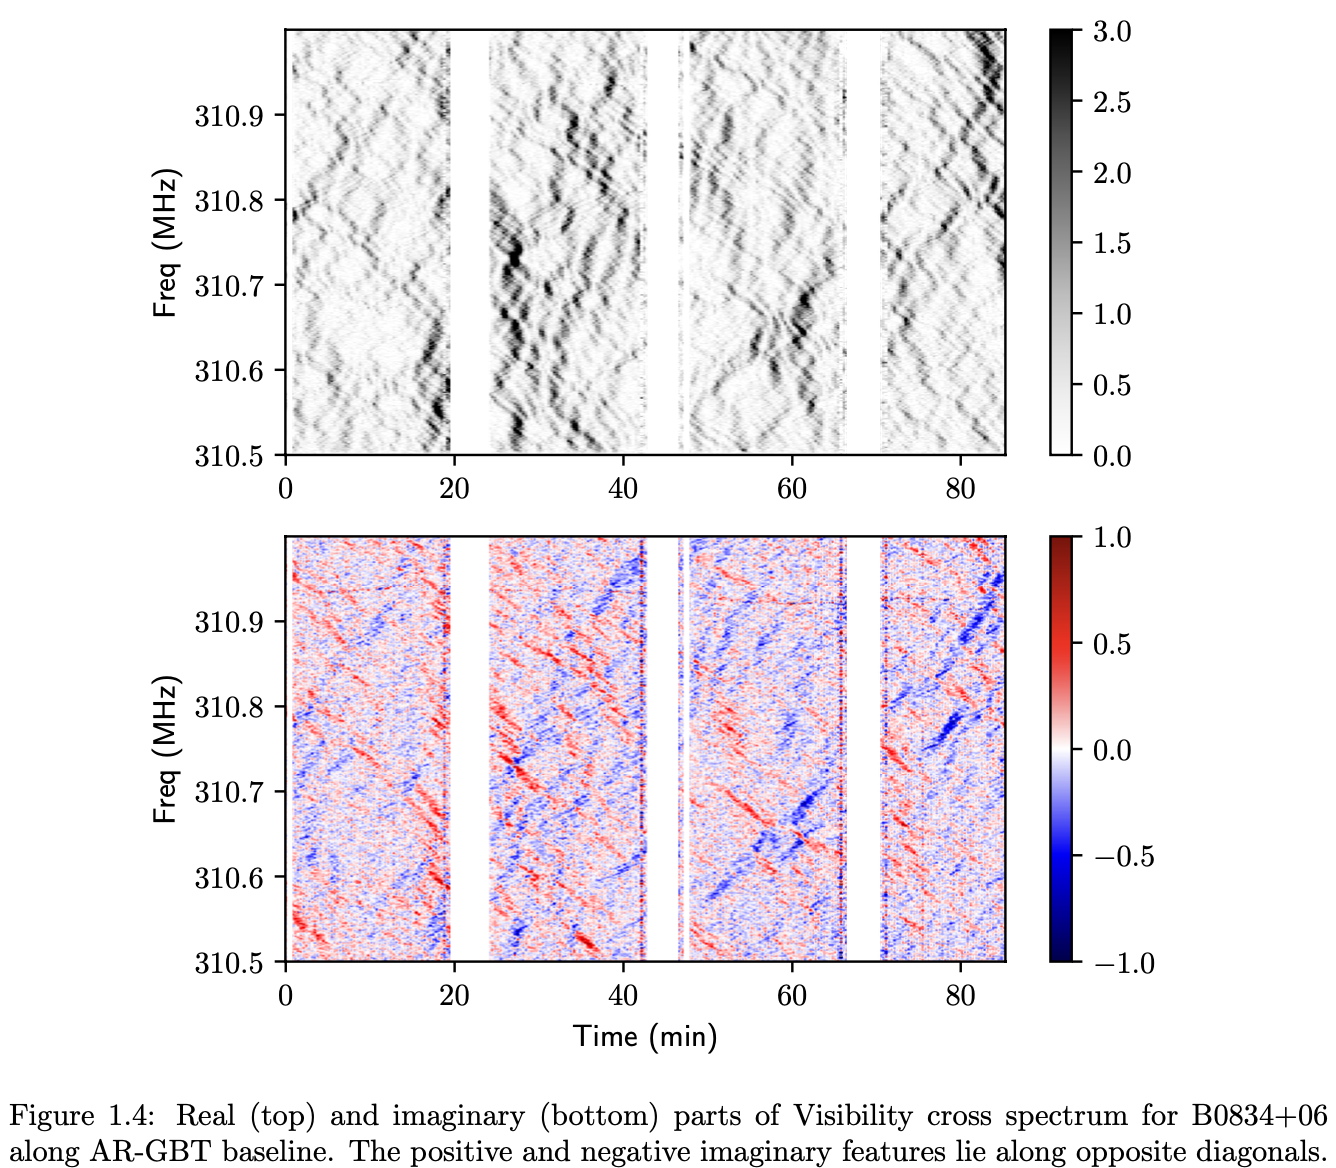
\includegraphics[width=3.25in]{Figures/rawvlbi.png}
\end{center}
  }
  \frame{
\vspace{-0.25in}
    \frametitle{Scintillometry VLBI}
\hspace{-0.25in}
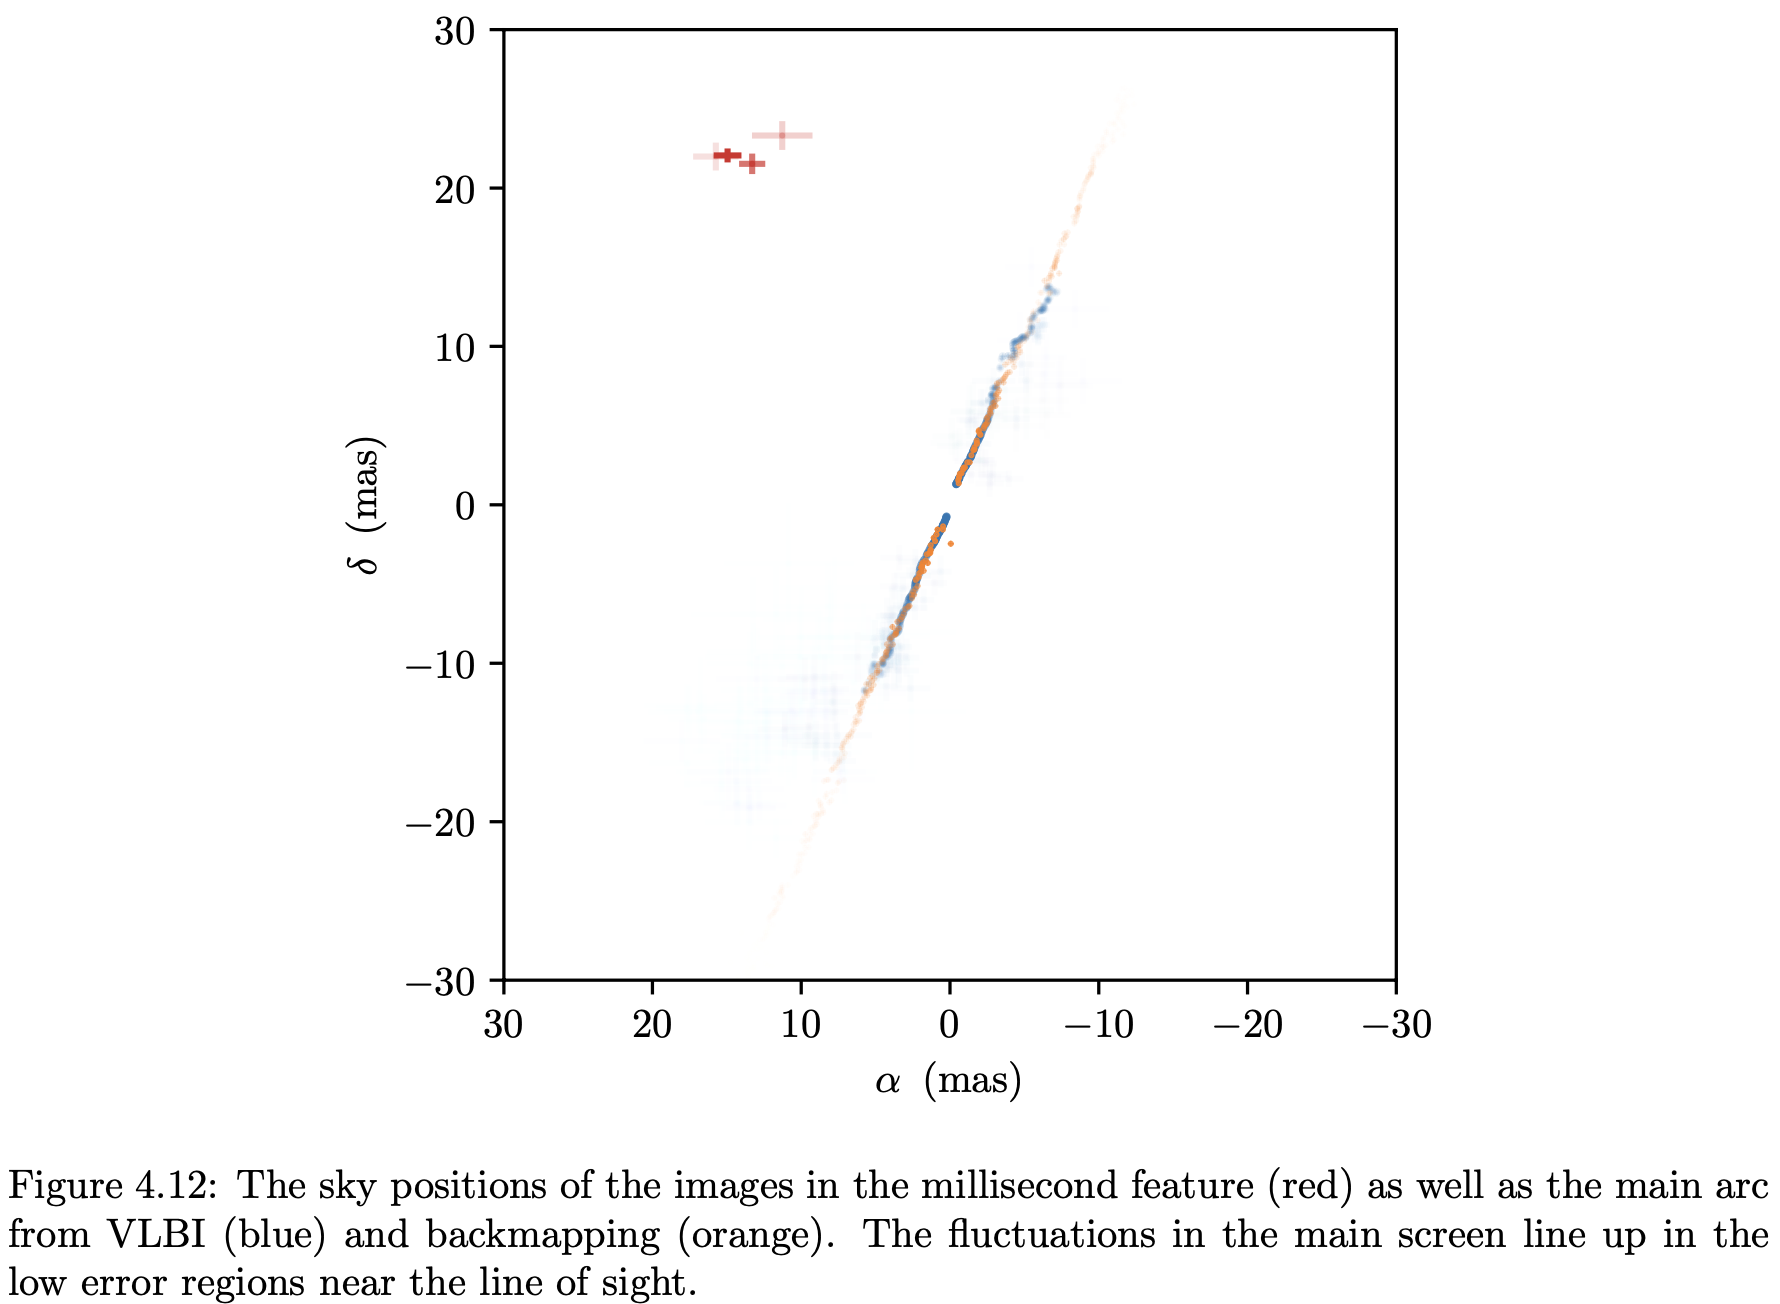
\includegraphics[width=3.5in]{Figures/VLBI0834.png}
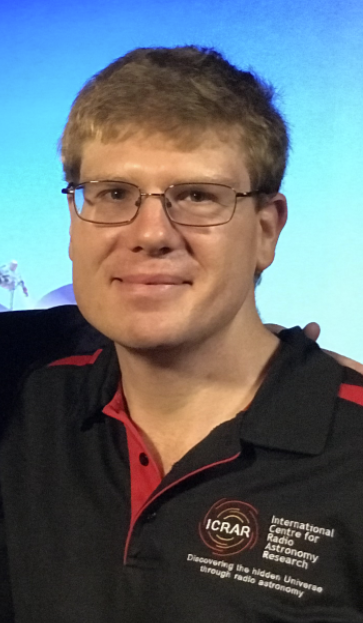
\includegraphics[width=1.05in]{Figures/jpm.png}
{\tiny
Baker++: increase PTA angular resolution to arcminutes.  In memoriam
J-P Macquart.
}
  }


  \frame{
    \frametitle{ISM Sheets}
    \begin{itemize}
      \item reconnection sheets
    \item grazing incidence
    \item ULP + King 2012
    \item ULP + Levin 2014
    \item Liu + ULP 2015
    \item 1-D structure
    \item localized scattering
%    \item predicts RM gradient
    \end{itemize}
\begin{picture}(320,235)
\put(110,170){
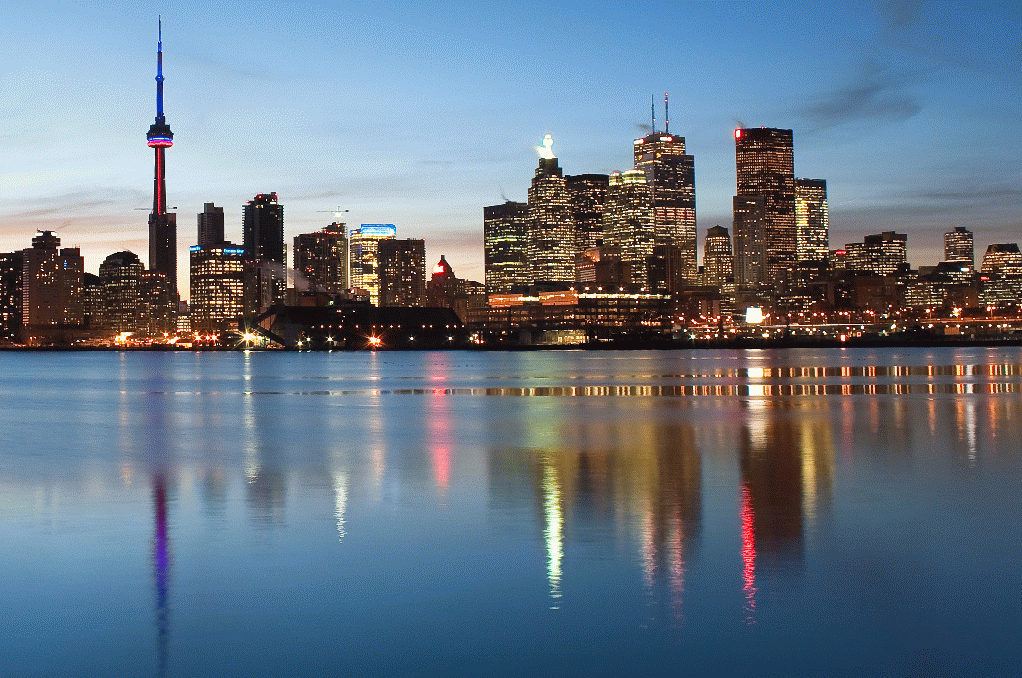
\includegraphics[width=3.0in]{Figures/toronto-skyline.png}}
\put(-60,-207){
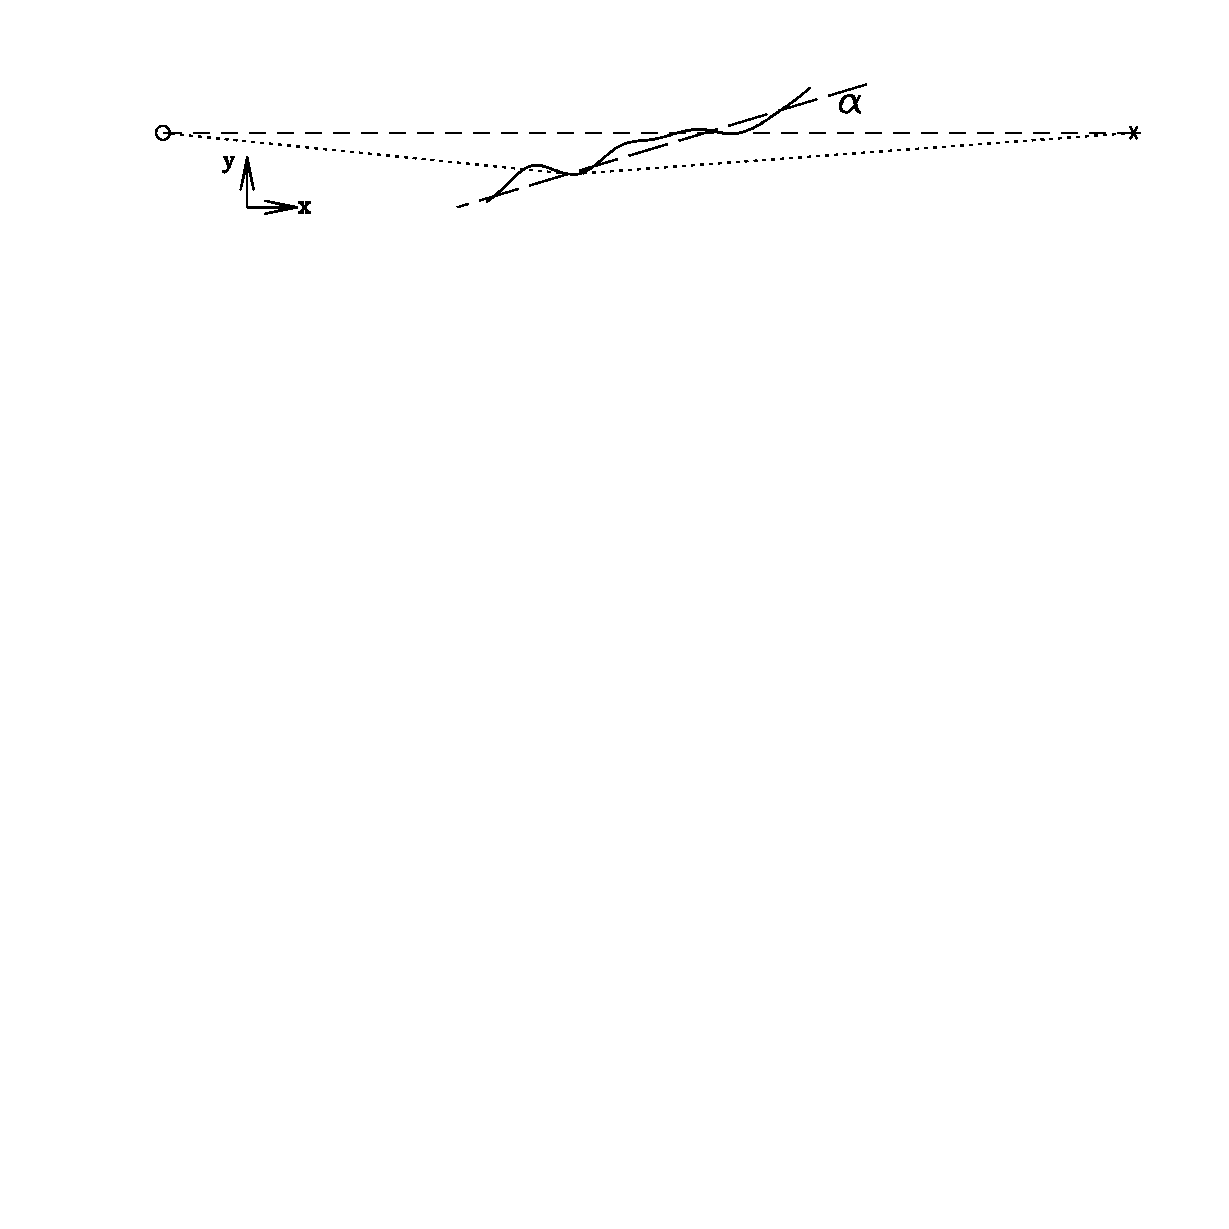
\includegraphics[width=5.5in]{Figures/sheetgeom.eps}}
\end{picture}
  }


  \frame{

    \frametitle{more precision astrometry}
%\vspace{-0.25in}
\begin{center}
%\hspace{-0.5in}
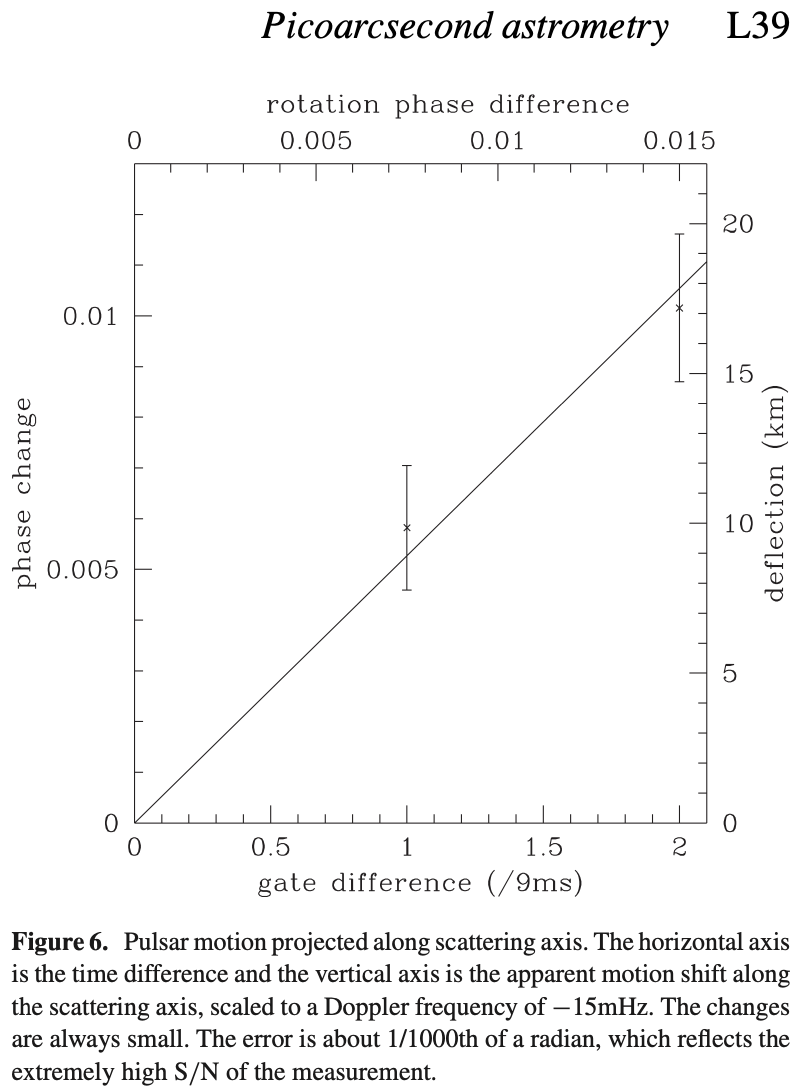
\includegraphics[width=2.05in]{Figures/pico.png}
UP+14
\end{center}
  }

 \frame{

    \frametitle{Hubble Constant}
%\vspace{-0.25in}
\begin{center}
%\hspace{-0.5in}
\includegraphics[width=2.05in]{Figures/frbh0.jpg}
Tsai, Jow, UP 2025
\end{center}
  }

 
  \frame{
%\vspace{-0.5in}
    \frametitle{New Observables}
    \begin{itemize}
    \item for coherent sources: FRBs, pulsars
    \item phase retrieval allows wave field mapping: analogous to radar
%    \item weak lensing: imaginary image allows time delay measurement (Jow+21)
    \item microlensing: instant time delay, planets (Jow+20)
    \item macrolensing: potentially nano-second delay -- universe
      expands!  Dark energy, etc (Wucknitz+21)
    \end{itemize}
  }


  \frame{

    \frametitle{Catastrophes: Exreme Scattering Events}
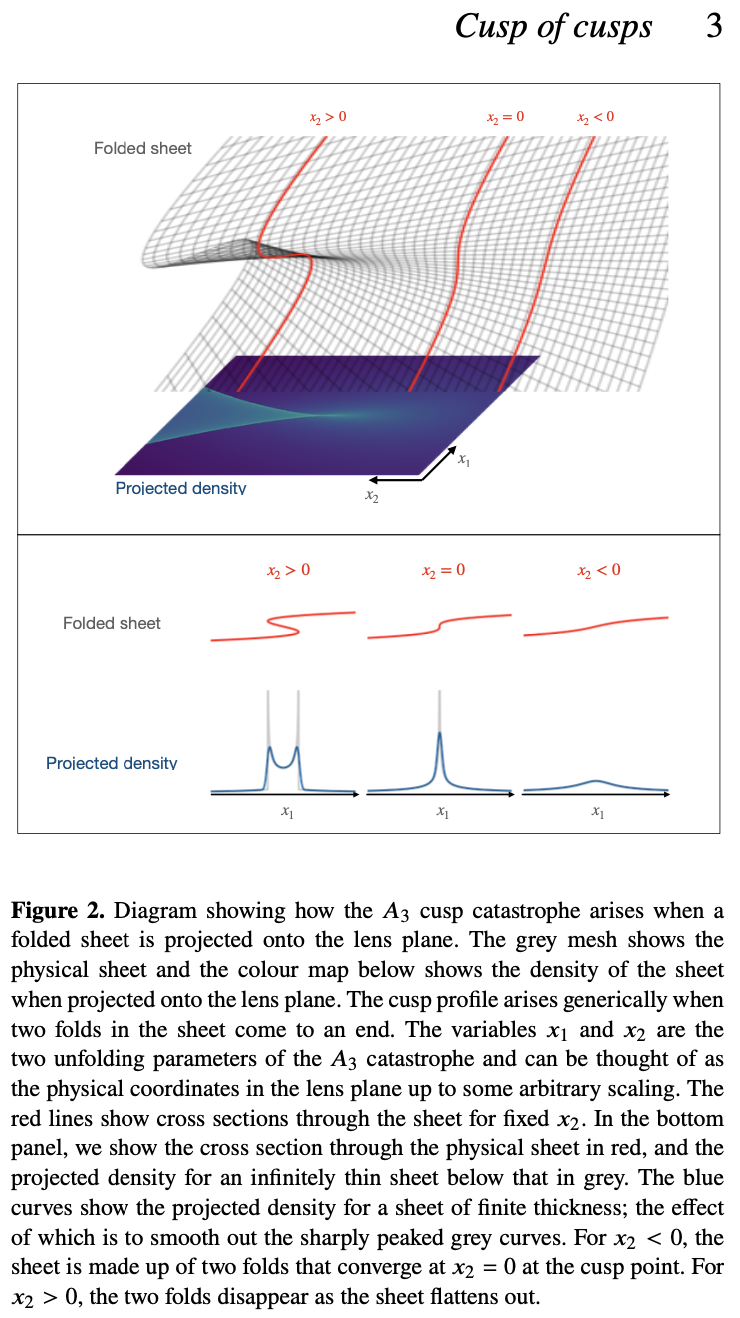
\includegraphics[width=2.85in]{Figures/cusp.png}
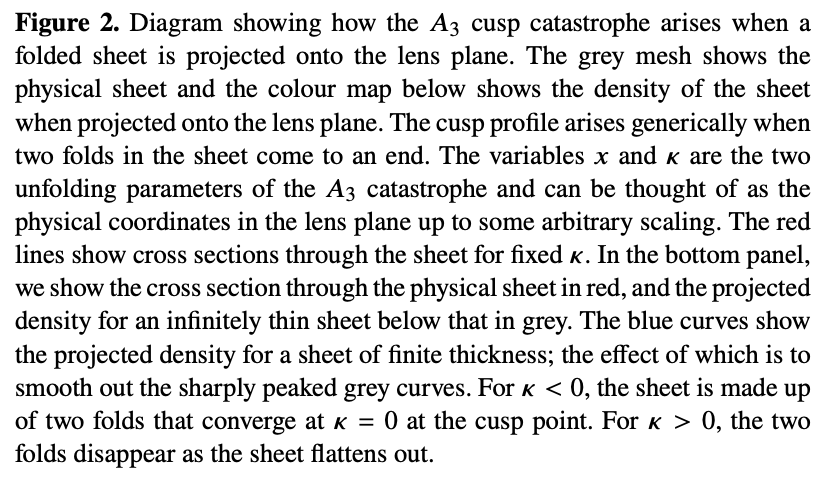
\includegraphics[width=0.5in]{Figures/cuspcaption.png}
Jow+2301.08344
  }

    \frametitle{Extreme Scattering Events}
%\hspace{-0.5in}
\vspace{0.5in}
\begin{center}
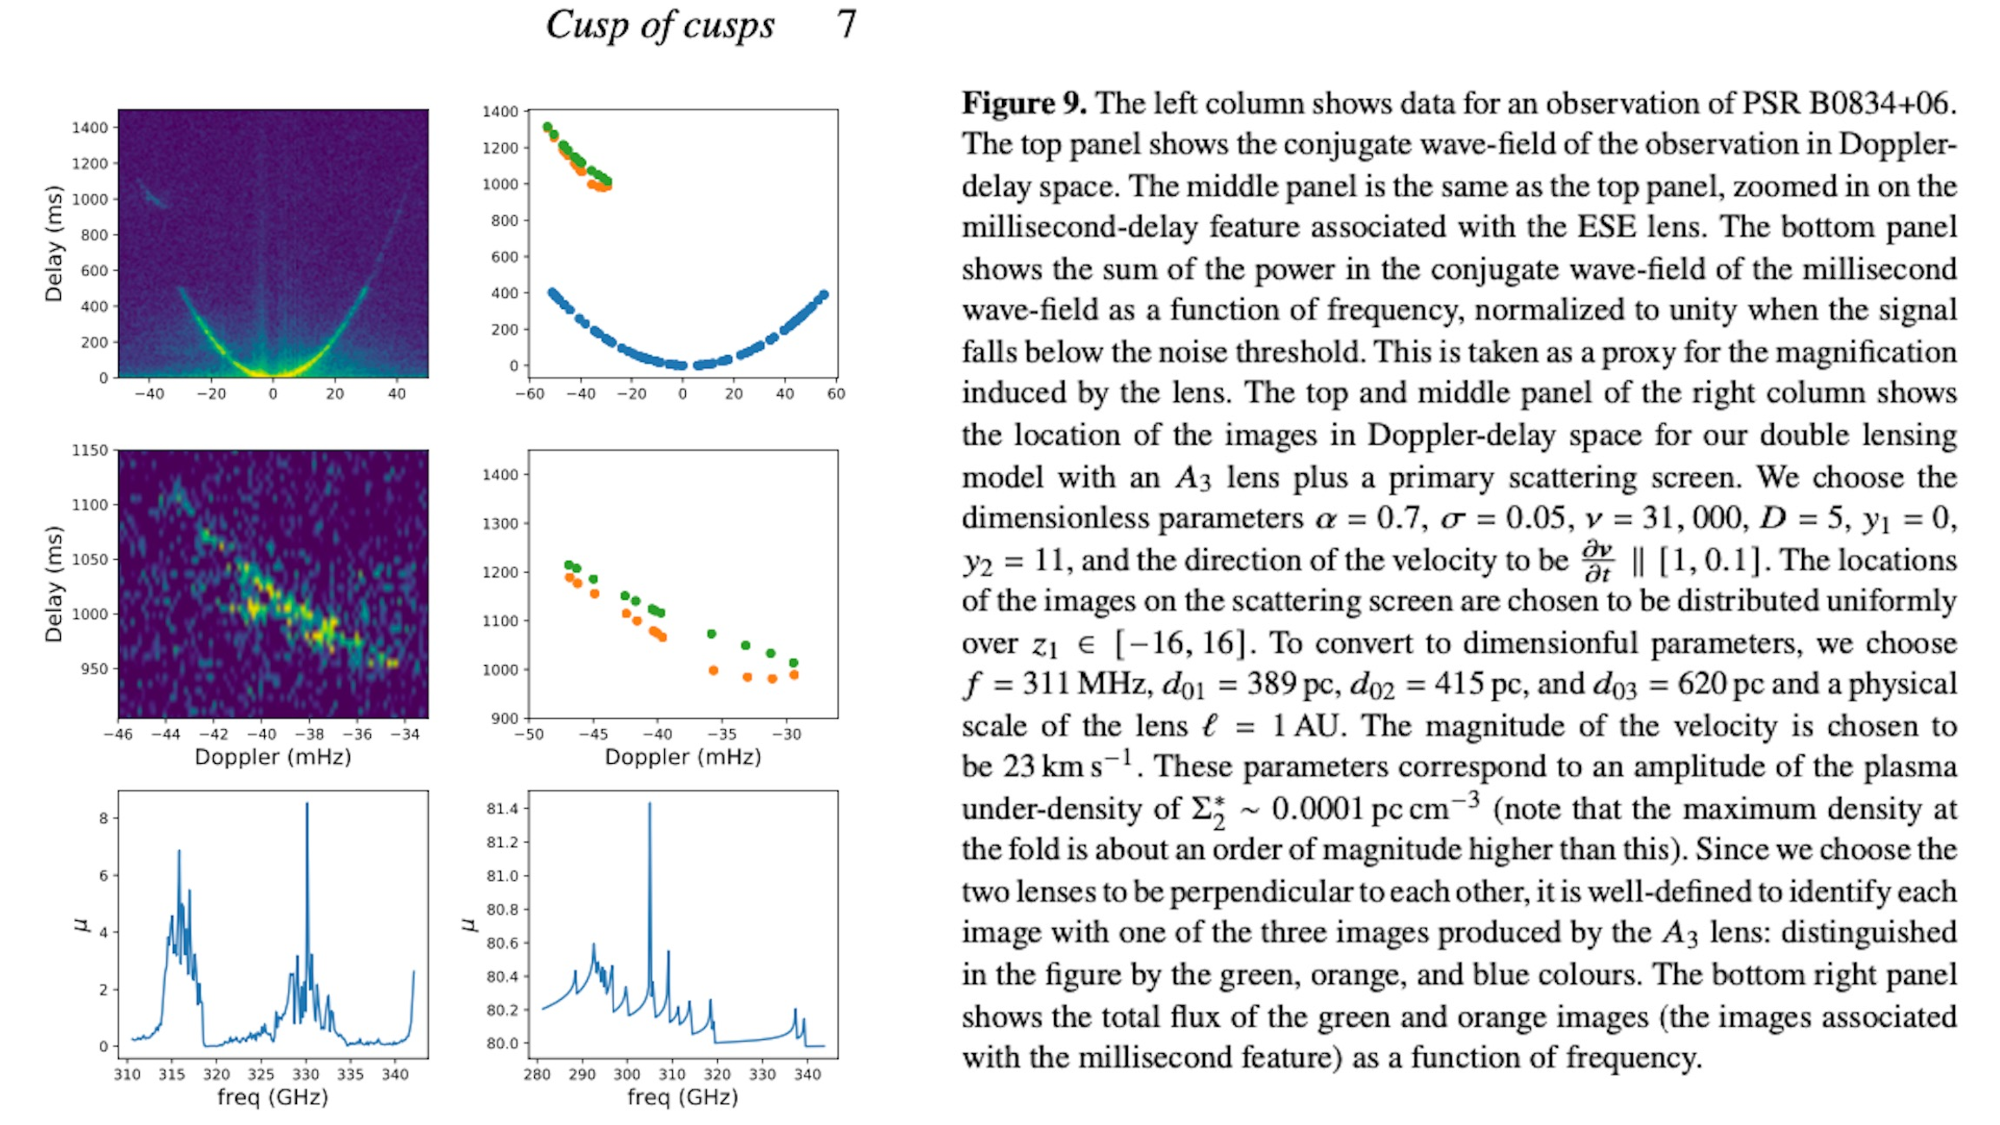
\includegraphics[width=4.65in]{Figures/esemodel.pdf}
\end{center}
  }


  \frame{
\vspace{-0.5in}
    \frametitle{Discussion}
    \begin{itemize}
    \item Eikonal effects applicable to compact radio sources,
      e.g. FRBs, pulsars
    \item full wave
effect dominates for long wavelengths as Fresnel scale is bigger then Einstein radius
    \item microlensing down to planet size
    \item gravitational waves:  LIGO, LISA, PTA
    \end{itemize}
  }
\section{BURSTT}

  \frame{
\vspace{-0.5in}
    \frametitle{BURSTT}
    \begin{itemize}
    \item Bustling Universe Radio Survey Telescope in Taiwan
    \item instant wide field, VLBI localization
    \item nearby counterparts, multi-wavelength, multi-messenger
    \item repeat statistics
    \item bright sample for deep followup
    \end{itemize}
  }


  \frame{
    \frametitle{BURSTT}
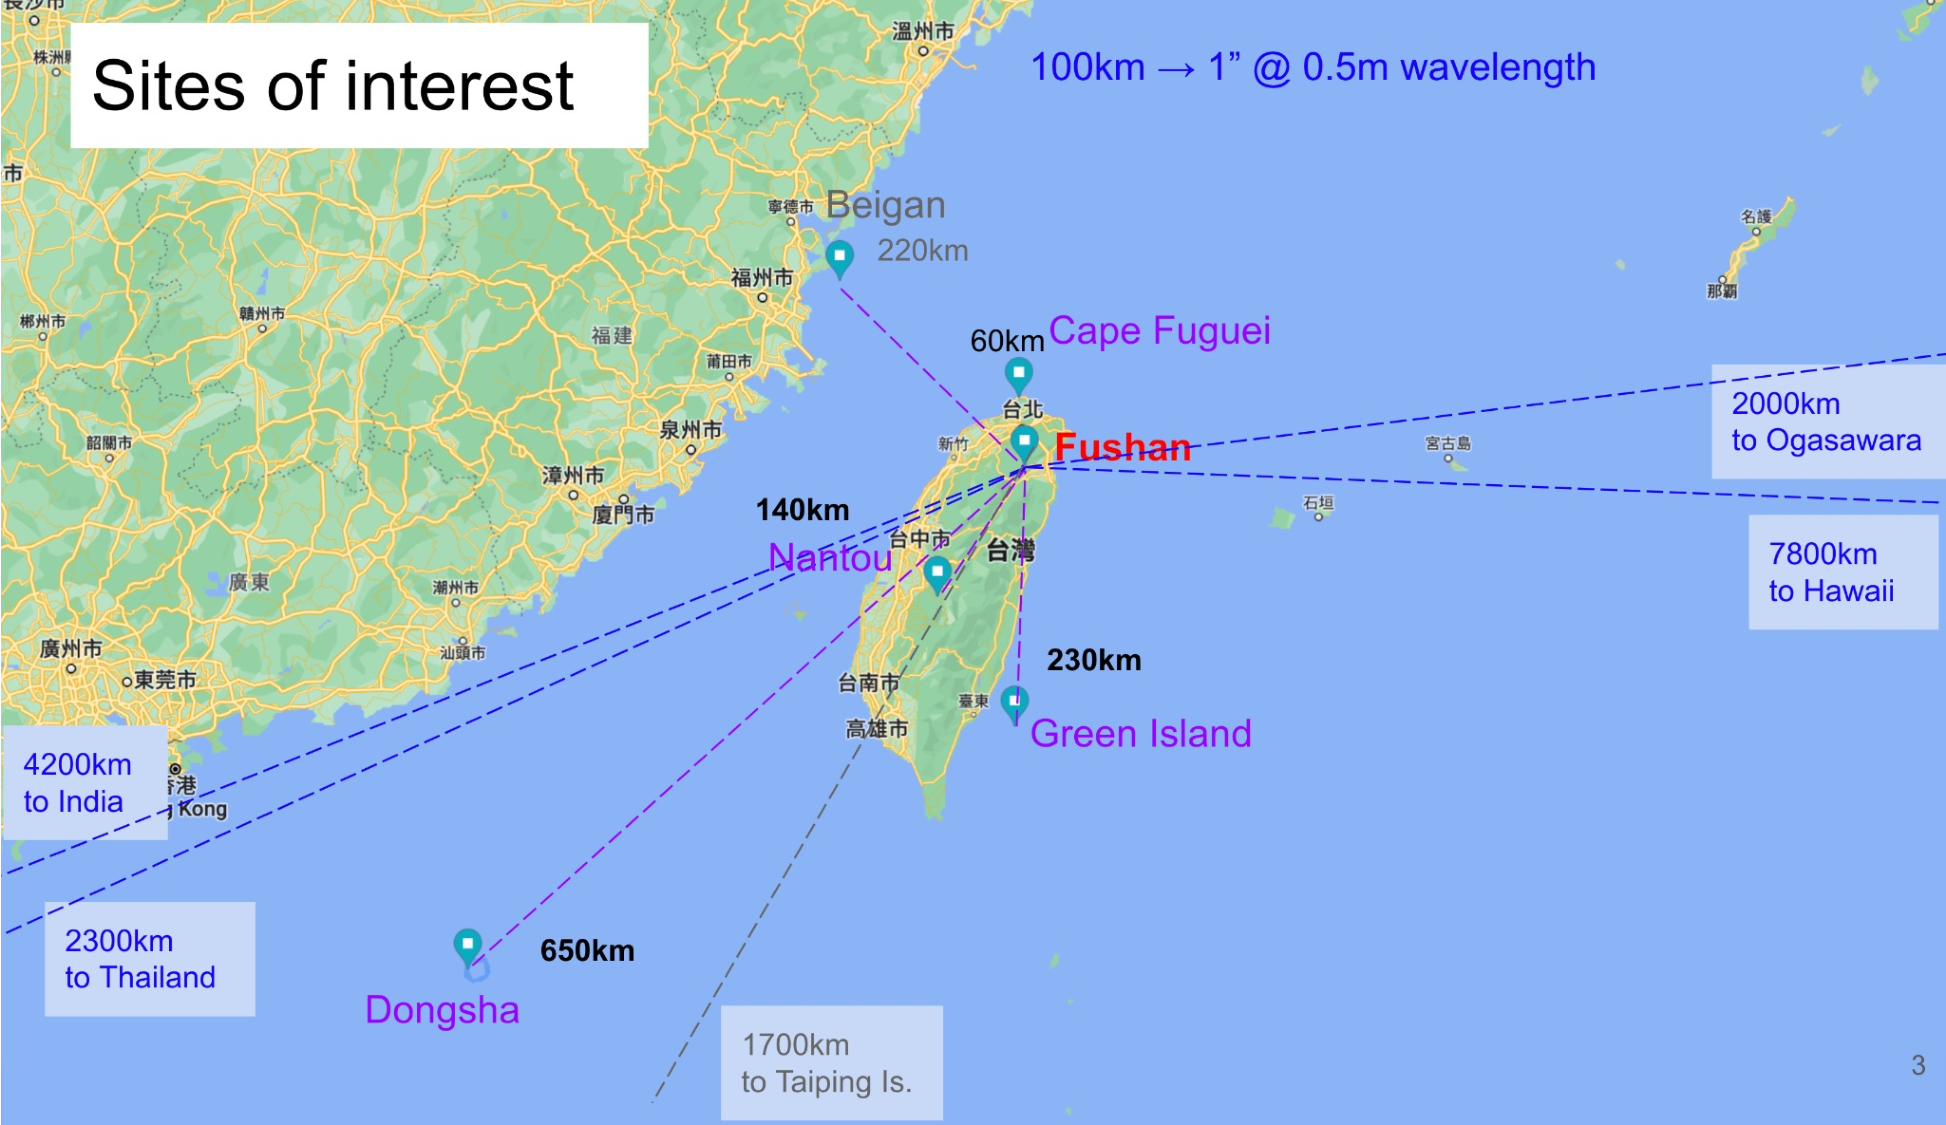
\includegraphics[width=4.5in]{Figures/bursttsites.pdf}
  }


  \frame{
    \frametitle{Fushan}
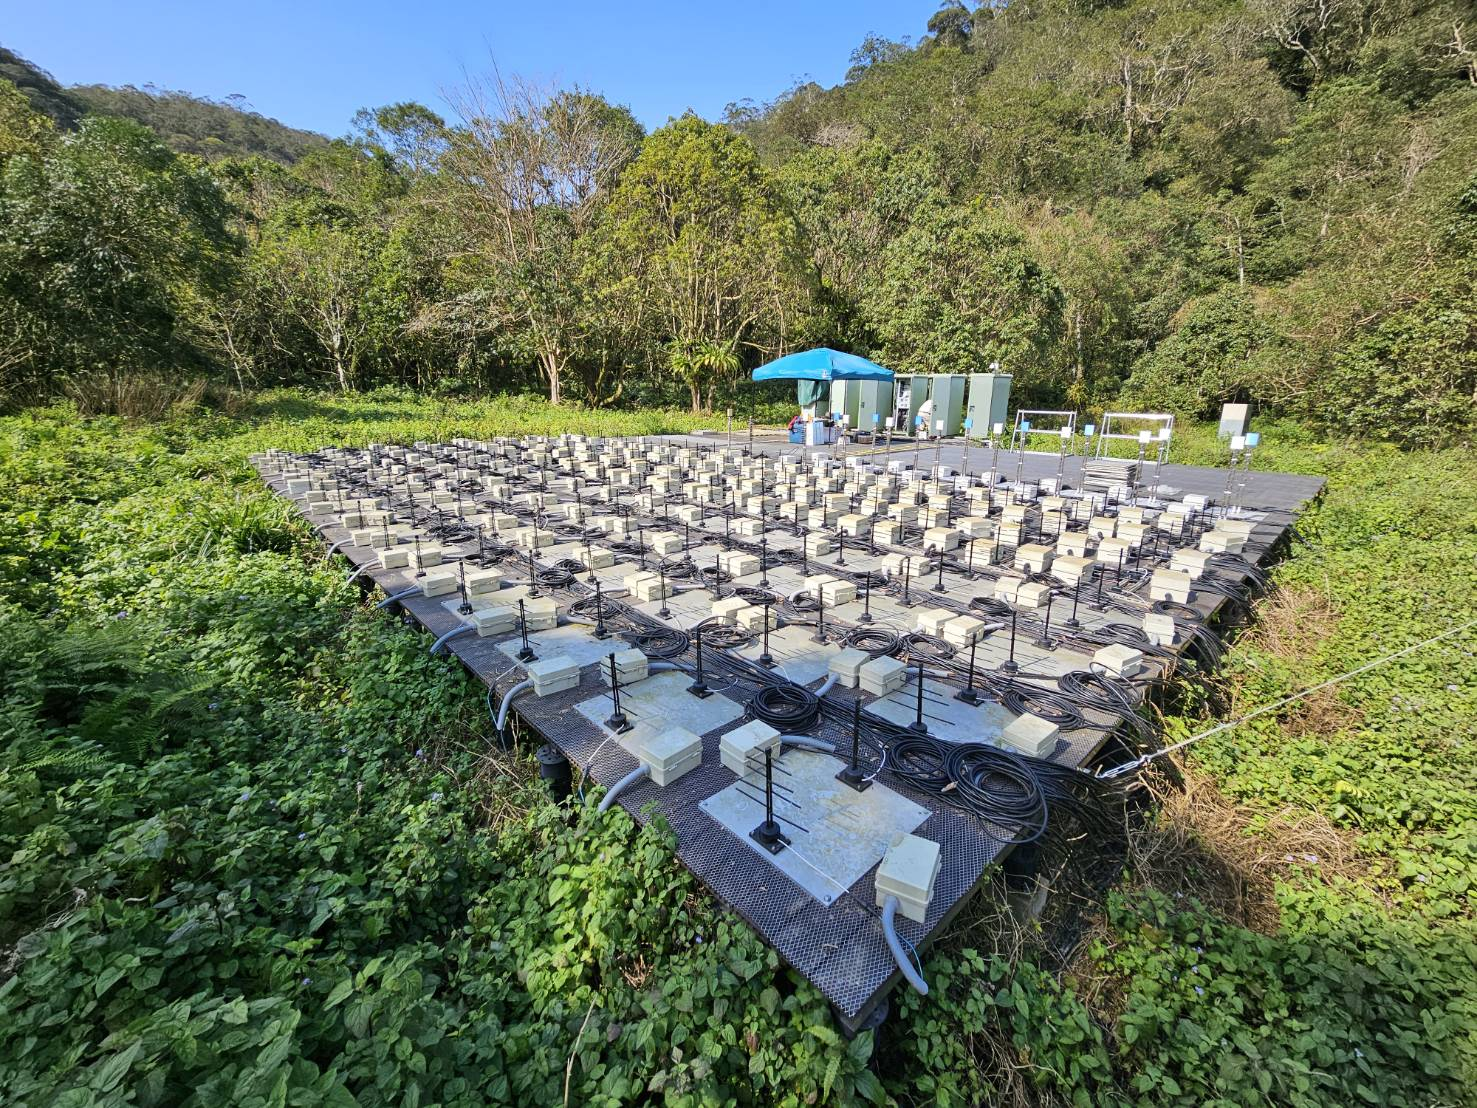
\includegraphics[width=4.5in]{Figures/fushan2025_1.jpg}
  }

  \frame{
    \frametitle{Nantou}
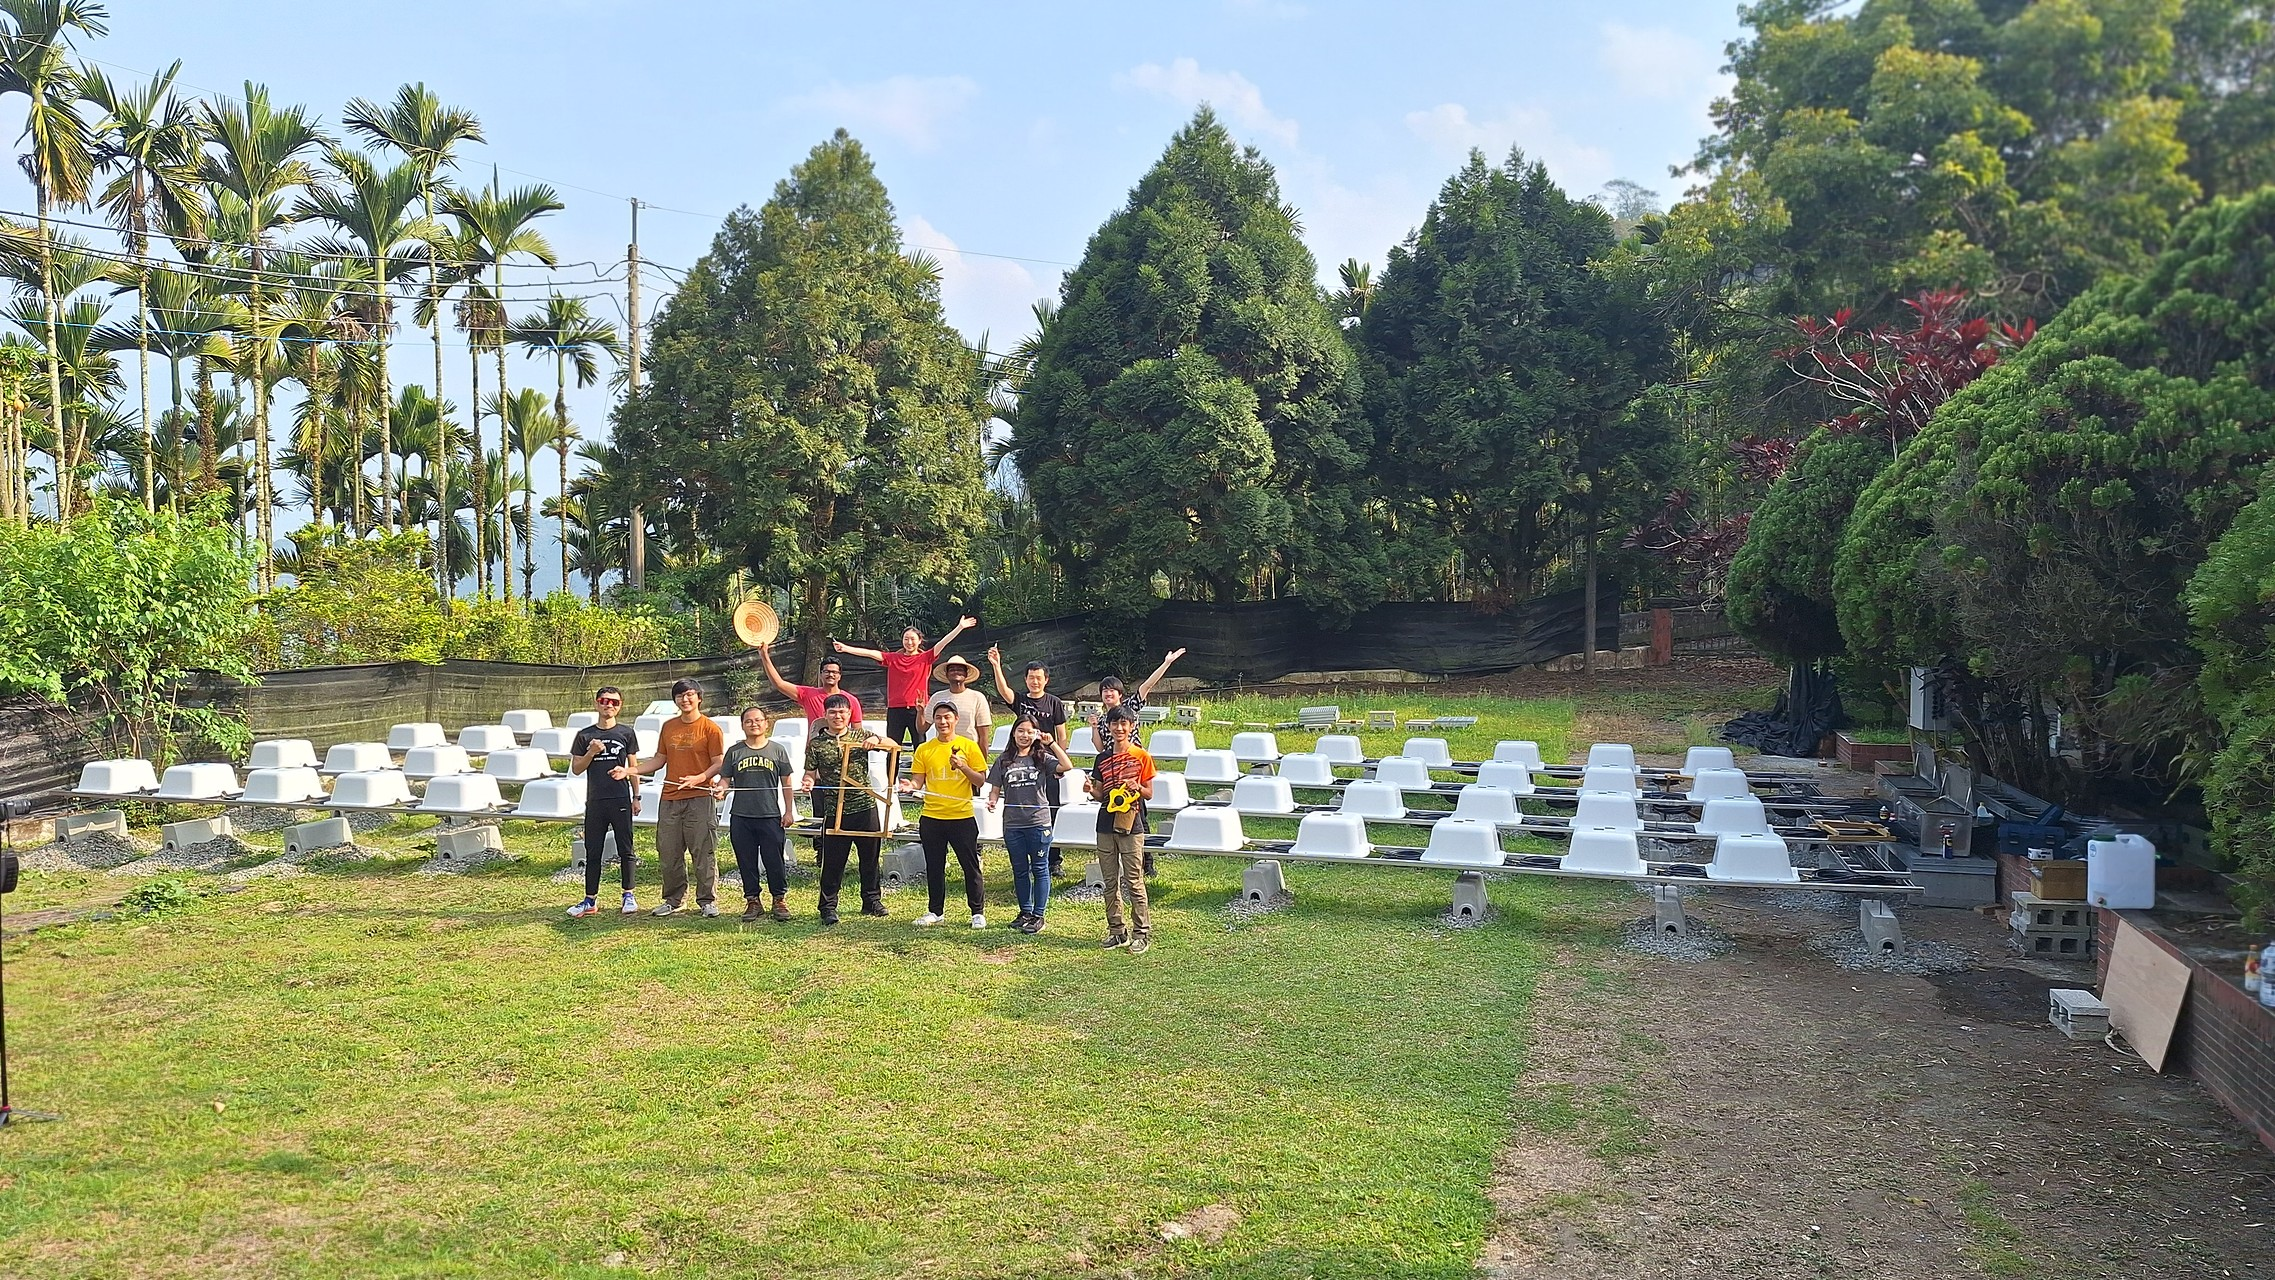
\includegraphics[width=4.5in]{Figures/nantou.JPEG}
  }


  \frame{
    \frametitle{Fugui}
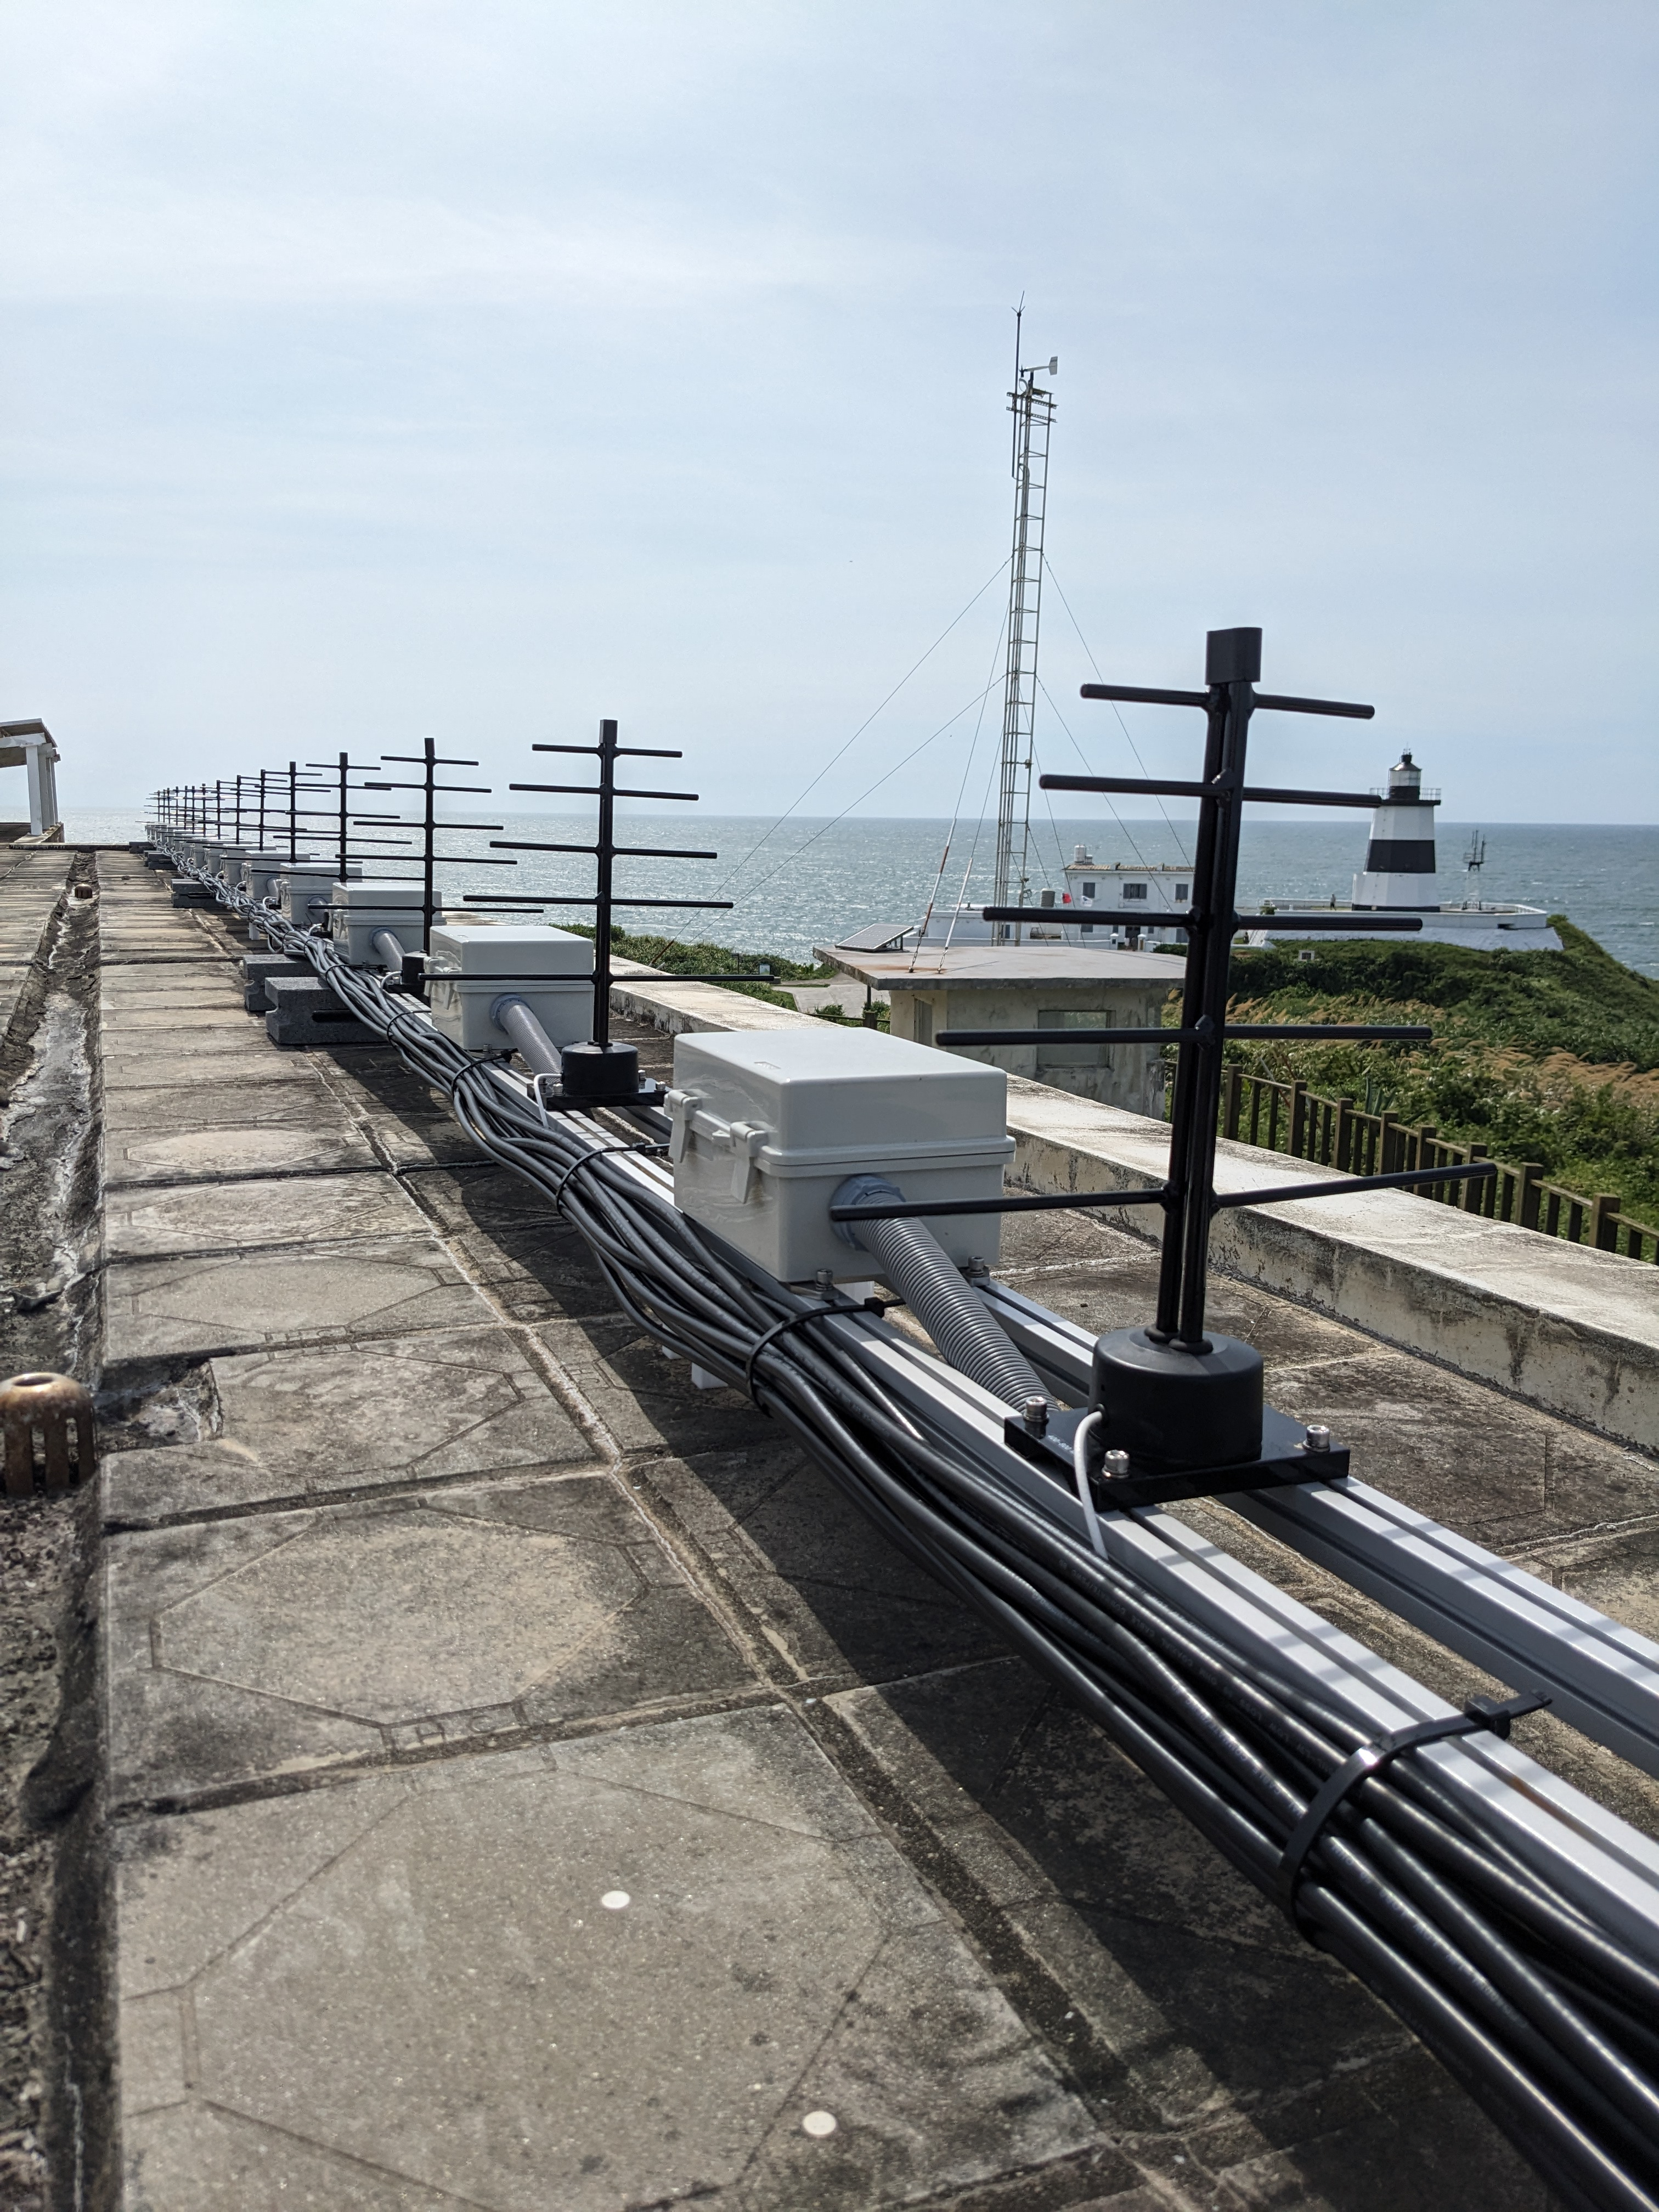
\includegraphics[width=2.5in]{Figures/bursttfugui.jpg}
  }

  \frame{
    \frametitle{Green Island}
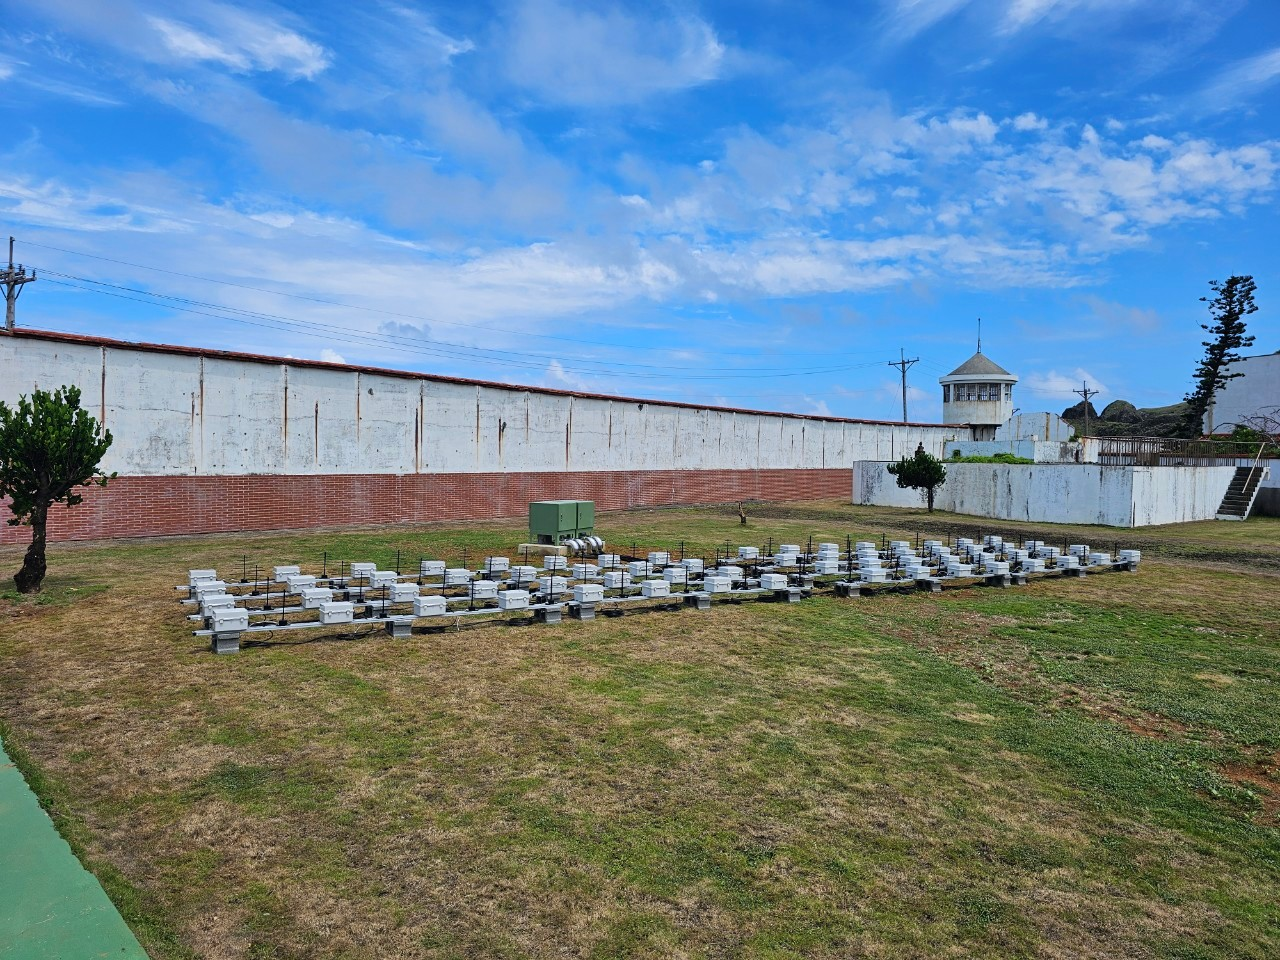
\includegraphics[width=4.5in]{Figures/ludao_250126_1.jpg}
  }

  \frame{
    \frametitle{Sun}
\movie[loop,width=3.5in]{sun}{Figures/map256_animate.gif}
  }

  \frame{
    \frametitle{VLBI}
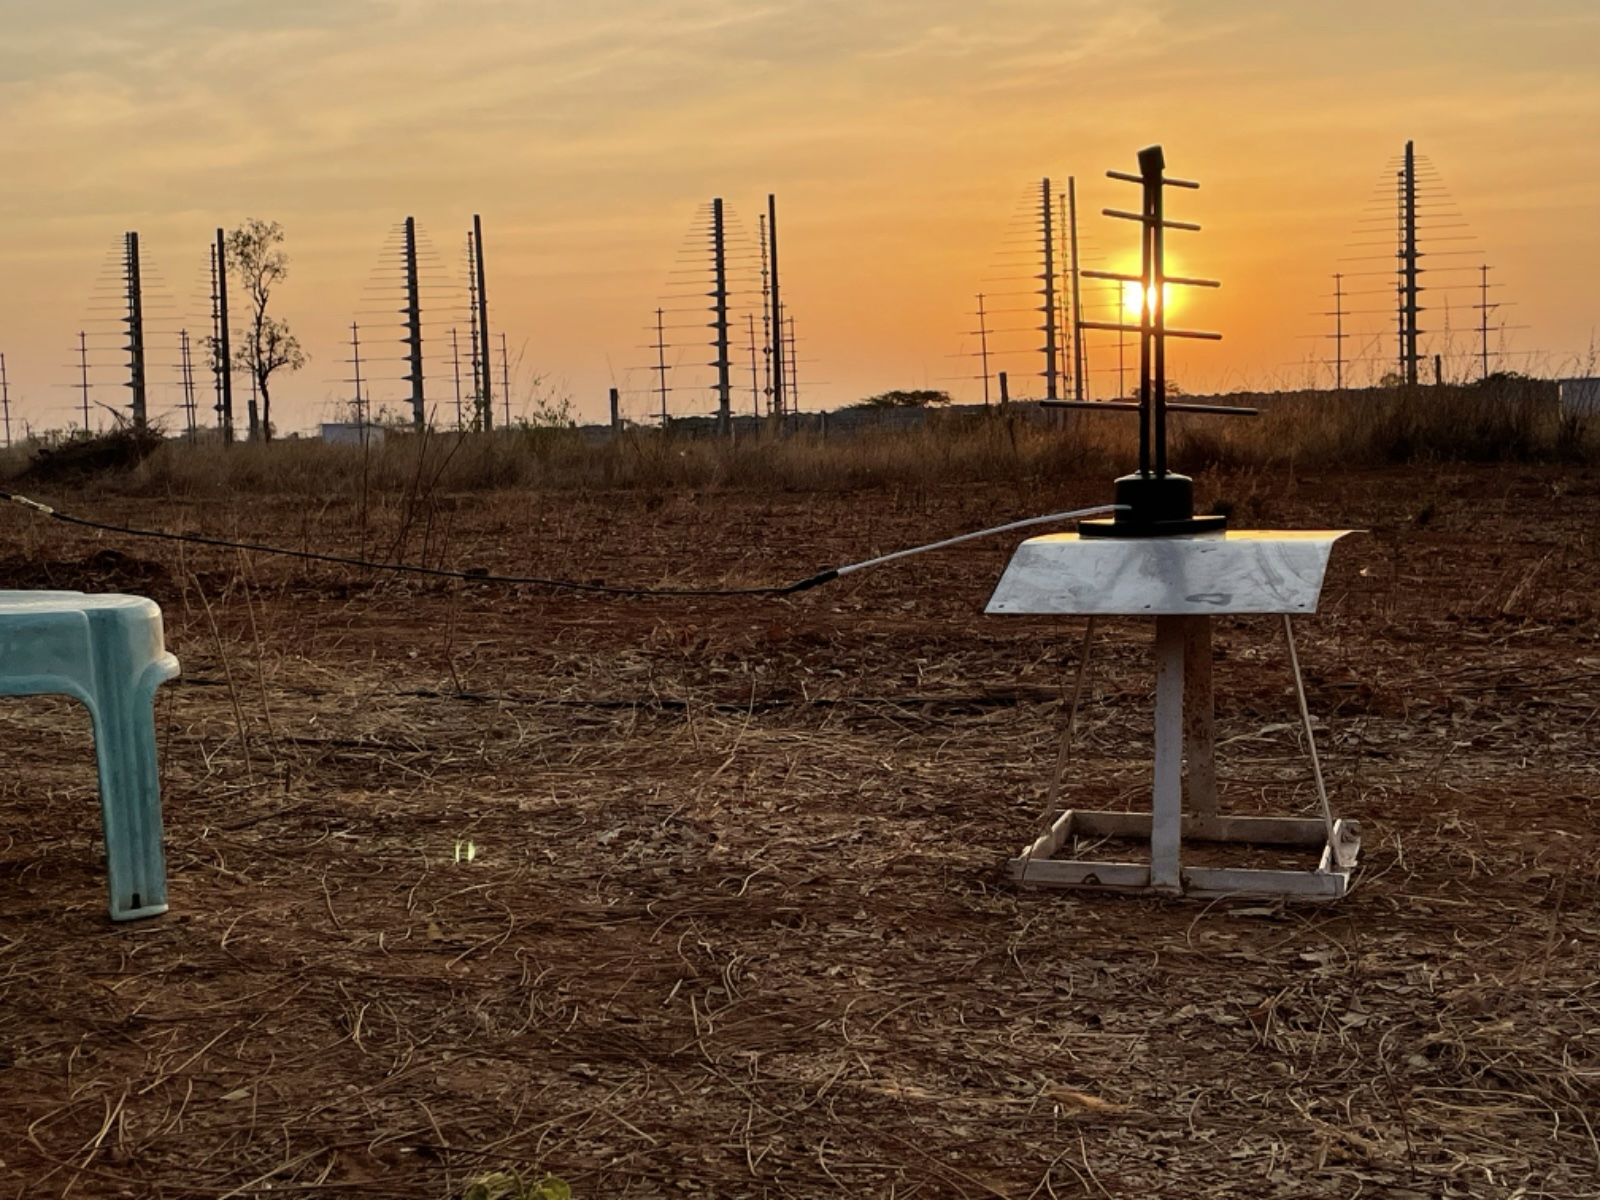
\includegraphics[width=1.95in]{Figures/gbd.jpg}
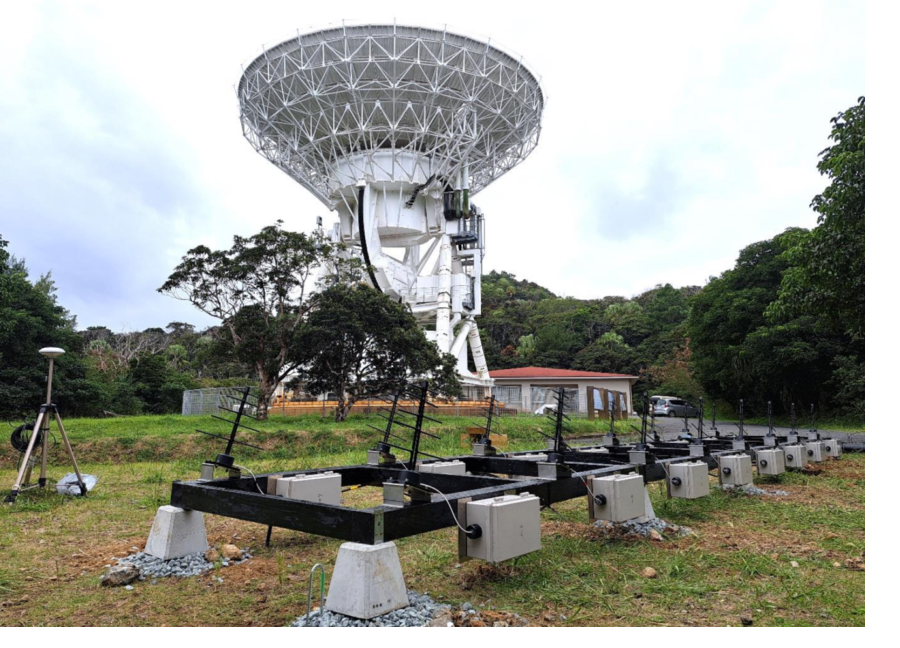
\includegraphics[width=1.95in]{Figures/ogasawara.jpg}

\includegraphics[width=3.5in]{Figures/intlmap.png}
  }


  \frame{
%\vspace{-0.5in}
    \frametitle{Conclusions}
    \begin{itemize}
     \item wave optics changes nature of astrophysical observables: Coherent FRB/pulsar/GW      radiation one of the potentially most
      precise measurements in physics
      \item already makes microarcsecond images of pulsars
      \item ISM plasma screens modelled quantitatively as localized
        1-D features, no longer stochastic turbulent volume.
      \item ESEs potentially arise from cusp folds, not from exploding
        dark matter or cosmic strings.
      \item next generation FRB telescopes for cosmic mass inventory,
        possibly dark energy/acceleration
 
      \item BURSTT completed phase 1 deployment, under commissioning
    \end{itemize}
  }

\end{document}
